In questo esperimento facoltativo si vuole realizzare un multi vibratore astabile basato su BJT che fa accendere alternativamente due diodi LED, ponendo particolare attenzione a comprenderne e descriverne il funzionamento. Il circuito è riportato in Figura \ref{fig:Circuit_fac}.Sono stati utilizzati i seguenti componenti:
\begin{itemize}
    \item 2 transistor bipolari NPN, codice BC548
    \item Resistenze: $R_1=R_4=470\Omega,R_2=R_3=47\text{k}\Omega$ 
    \item Condensatori: $C_1=C_2=10\mu F$
    \item LED rossi, codice CREE C503B-RCS-CW0Z0AA1
\end{itemize}
Il circuito è alimentato da una tensione $V_{CC}=+12V$ e in Figura \ref{fig:Package3} si è riportato il package del transistor e del led
\begin{figure}[H]
    \centering
    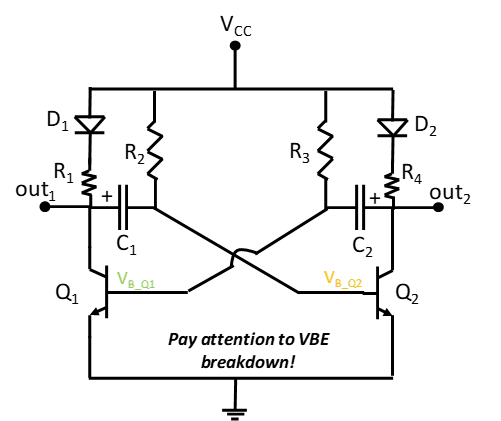
\includegraphics[width=0.5\linewidth]{images/Circuit_fac1.png}
    \caption{Schema circuito}
    \label{fig:Circuit_fac}
\end{figure}
\begin{figure}[H]
    \centering
    \begin{subfigure}{.5\textwidth}
      \centering
      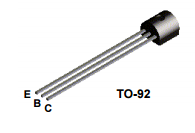
\includegraphics[width=0.5\linewidth]{images/BC548.png}
    \end{subfigure}%
    \begin{subfigure}{.5\textwidth}
      \centering
      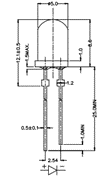
\includegraphics[width=0.3\linewidth]{images/LED.png}
    \end{subfigure}
    \caption{Package del BJT BC548 e del LED}
    \label{fig:Package3}
\end{figure}

\subsection{Risultati}
\subsubsection*{Misurare le forme d’onda alla base e al collettore del transistor $Q_1$ e riportarle in relazione}
Con l'utilizzo dell'oscilloscopio è stato campionato il segnale e  ottenuto le seguenti forme d'onda, riportate in Figura \ref{fig:FacBaseQ1} per la misura alla base e in Figura \ref{fig:FacCollectorQ1} per la misura al collettore.
\begin{figure}[H]
    \centering
    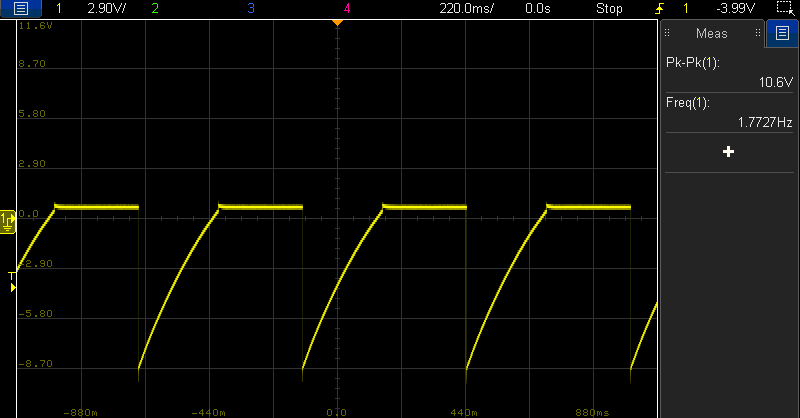
\includegraphics[width=0.7\linewidth]{images/scope_20.png}
    \caption{Forma d'onda campionata alla base di $Q_1$}
    \label{fig:FacBaseQ1}
\end{figure}
\begin{figure}[H]
    \centering
    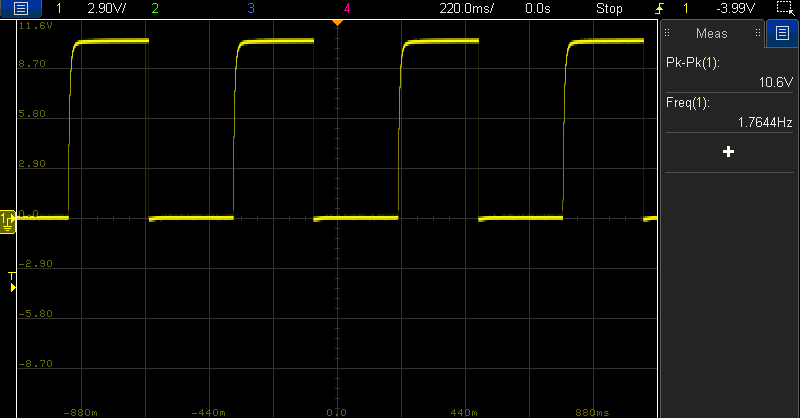
\includegraphics[width=0.7\linewidth]{images/scope_22.png}
    \caption{Forma d'onda campionata al collettore di $Q_1$}
    \label{fig:FacCollectorQ1}
\end{figure}
\subsubsection*{Riportare il confronto della forma d’onda $out_1$ e $out_2$ in relazione}
Sempre con l'utilizzo dell'oscilloscopio è stato campionato il canale di entrambe le uscite per poi metterle a confronto in Figura \ref{fig:FacConfronto}
\begin{figure}[H]
    \centering
    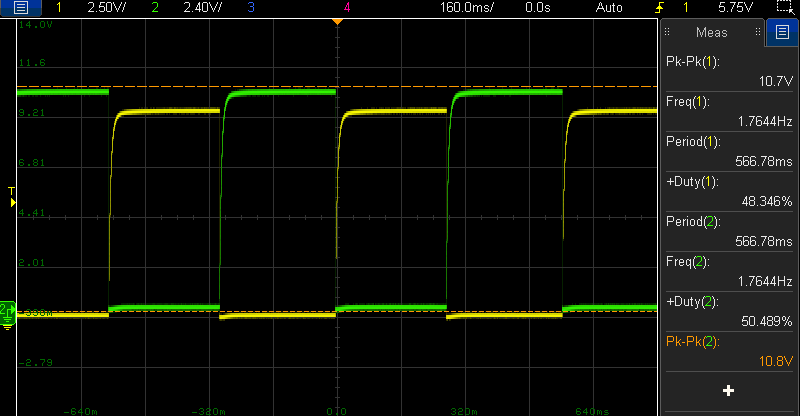
\includegraphics[width=0.7\linewidth]{images/scope_26.png}
    \caption{Confronto della forma d’onda $out_1$ e $out_2$}
    \label{fig:FacConfronto}
\end{figure}
\subsubsection*{Valutare il periodo, frequenza e duty cycle della forma d’onda generata all’uscita $out_1$ e $out_2$}
L'oscilloscopio fornisce i seguenti parametri delle forme d'onda generate dal circuito, riassunti nella Tabella \ref{tab:RisFac1}
\begin{table}[H]
    \centering
    \begin{tabular}{||c|c|c|c|c||}
        \hline\hline
        Uscita & Vpp & Periodo & Frequenza & Duty cycle \\\hline
        $out_1$ & 10.7V & 566.78ms & 1.7644Hz & 48.346\% \\\hline
        $out_2$ & 10.8V & 566.78ms & 1.7644Hz & 50.489\%\\\hline
    \end{tabular}
    \caption{Valutazione dei segnali di uscita}
    \label{tab:RisFac1}
\end{table}
\subsection{Funzionamento del circuito} 

Un circuito multivibratore astabile basato su transistor BJT è costituito da due BJT, due condensatori, due diodi e quattro resistenze, tali che $R_1=R_2<R_2=R_3$. Il circuito funziona in modo che i due transistor si alternino nel loro stato di accensione e spegnimento. Entrambi i transistor sono accoppiati a croce, ciò significa che il collettore di un transistor è connesso alla base dell'altro transistor attraverso una capacità.
Nel momento in cui viene fornita l'alimentazione, uno dei due transistor si accende più rapidamente dell'altro a causa di piccole differenze tra i dispositivi. Supponendo che $Q_1$ vada in saturazione per primo, la tensione base-emettitore di $Q_1$ si porta al valore di $0.7V$ e la tensione al collettore di $Q_2$ si porta al potenziale di massa. Questo comporta che alla base di $Q_2$ appare l'inverso della tensione ai capi del condensatore $C_1$, portandolo nella regione di interdizione (cut-off), di conseguenza al collettore di $Q_2$ si ha il potenziale $V_{cc}$. 
Si ha $Q_1$ On e $Q_2$ Off.\\\\
Il condensatore $C_2$ inizia a caricarsi fino al potenziale $V_{cc}-V_{be}$, mentre il condensatore $C_1$ fino a $V_{cc}$. Dato $R_1<R_2$ si ha che $C_2$ si carica più rapidamente di $C_1$.
Appena la tensione ai capi di $C_1$ (e quindi alla base di $C_2$) diventa $0.7V$ il transistor $Q_2$ inizia a condurre fino a entrare in saturazione. Di conseguenza la tensione al collettore di $Q_2$ si porta al potenziale di massa. La tensione alla base di $Q_1$ si porta all'inverso del valore ai capi di $C_2$, quindi a $-(V_{cc} - V_{be})$ e $Q_1$ entra in interdizione.
Si ha $Q_1$ Off e $Q_2$ On.\\\\
Da qui in poi il circuito continuerà a cambiare tra i due stati fino alla rimozione dell'alimentazione.
\subsection{Periodo della forma d’onda}
Il periodo $T$ della forma d'onda dipende dalle resistenze $R_2$ e $R_3$ e dai condensatori $C_1$ e $C_2$ utilizzati nel circuito, secondo la formula:
\begin{equation}
    T=\ln{2}(R_2C_1+R_3C_2)
\end{equation}
